\section{Реализация и результаты}
\label{sec:work}

\subsection{Модель рекуррентной сети}

Задача прогнозирования решается в следующей постановке. Ряд $\{x_t\}_{t=1}^{N}$ ($N \ge 10$) нормализуется в диапазон $[-1, 1]$:
\begin{equation}
	\tilde{x}_t = 2\,\frac{x_t - x_{\min}}{x_{\max} - x_{\min}} - 1.
\end{equation}
На каждом шаге $t$ сеть получает входной скаляр $\tilde{x}_t$ и текущий вектор контекста $c_t$; скрытый слой формирует вектор $h_t$, а эффекторный (выходной) нейрон выдаёт прогноз $y_t \approx \tilde{x}_{t+1}$:
\begin{equation}
	h_t = f\bigl(W_{xh}\,[\,\tilde{x}_t;\, c_t\,] + W_{hh}\,h_{t-1} + b_h\bigr), \qquad
	y_t = g\bigl(W_{ho}\,h_t + b_o\bigr).
\end{equation}
Конкретный вид связи, формирующей контекст $c_{t+1}$, и состав матриц $W_{xh}, W_{hh}$ определяют архитектуру сети.

\subsubsection{Архитектуры}

\textbf{Сеть Элмана.} Контекст формируется из скрытого слоя (одна задержка):
\begin{equation}
	c_{t+1} = h_t[:C].
\end{equation}

\textbf{Сеть Джордана.} Контекст формируется из выхода эффектора (линия задержки):
\begin{equation}
	c_{t+1} = [\,y_t;\; c_t[:C-1]\,].
\end{equation}

\textbf{Сеть Джордана~--~Элмана.} Контекст объединяет оба источника: первые $C_e$ компонент~\mdash  из скрытого слоя, оставшиеся $C_j$~\mdash  из выхода:
\begin{equation}
	c_{t+1} = [\,h_t[:C_e];\; y_t;\; c_t[C_e{:}C_e{+}C_j{-}1]\,], \qquad C_e + C_j = C.
\end{equation}

\textbf{Простая рекуррентная сеть (КП).} Скрытое состояние поддерживается рекуррентной связью $W_{hh}$, отдельного контекста нет ($c_t \equiv 0$):
\begin{equation}
	h_t = f\bigl(W_{xh}\,\tilde{x}_t + W_{hh}\,h_{t-1} + b_h\bigr).
\end{equation}

\textbf{Сеть с долговременной кратковременной памятью (LSTM, ДКП).} Вместо одного вектора состояния поддерживаются скрытое $h_t$ и ячейное $c_t$ состояния; три ворота (входное $i$, забывающее $f$, выходное $o$) и кандидат $g$:
\begin{align}
	z_t &= W_{xh}\,\tilde{x}_t + W_{hh}\,h_{t-1} + b, \\
	i_t &= \sigma(z_t^{i}), \quad f_t = \sigma(z_t^{f}), \quad o_t = \sigma(z_t^{o}), \quad \tilde{c}_t = \tanh(z_t^{g}), \\
	c_t &= f_t \odot c_{t-1} + i_t \odot \tilde{c}_t, \\
	h_t &= o_t \odot \tanh(c_t),
\end{align}
где $\sigma(\cdot)$~\mdash  сигмоида, $\odot$~\mdash  поэлементное умножение. Согласно методическим указаниям, функция активации эффектора~\mdash  экспоненциальная линейная (ELU).

\textbf{Сеть с управляемыми рекуррентными блоками (GRU).} Два ворота (обновления $z$ и сброса $r$):
\begin{align}
	z_t &= \sigma\bigl(W_{xz}\,\tilde{x}_t + W_{hz}\,h_{t-1} + b_z\bigr), \\
	r_t &= \sigma\bigl(W_{xr}\,\tilde{x}_t + W_{hr}\,h_{t-1} + b_r\bigr), \\
	\tilde{h}_t &= \tanh\bigl(W_{xh}\,\tilde{x}_t + W_{hh}\,(r_t \odot h_{t-1}) + b_h\bigr), \\
	h_t &= (1 - z_t) \odot h_{t-1} + z_t \odot \tilde{h}_t.
\end{align}
Эффектор также использует ELU.

\subsubsection{Функции активации}

Скрытый слой может использовать одну из четырёх функций (и их производные, используемые при обратном распространении):
\begin{align}
	\text{арксинус:} & \quad f(u) = \operatorname{arcsinh}(u), & f'(u) &= \frac{1}{\sqrt{1+u^2}}, \\
	\text{тангенс:} & \quad f(u) = \tanh(u), & f'(u) &= 1 - \tanh^2(u), \\
	\text{ELU:} & \quad f(u) = \begin{cases} u, & u \ge 0, \\ \alpha (e^{u} - 1), & u < 0, \end{cases} & f'(u) &= \begin{cases} 1, & u \ge 0, \\ \alpha e^{u}, & u < 0, \end{cases} \\
	\text{Leaky ReLU:} & \quad f(u) = \begin{cases} u, & u \ge 0, \\ a\,u, & u < 0, \end{cases} & f'(u) &= \begin{cases} 1, & u \ge 0, \\ a, & u < 0, \end{cases}
\end{align}
где $\alpha = 1$, $a = 0{,}01$. Для эффектора опционально задаётся линейная активация $g(u) = u$ (для LSTM и GRU по методичке~\mdash  ELU).

\subsubsection{Обучение и многомерный прогноз}

Обучение~\mdash  обратное распространение во времени (BPTT) по окну длины $w$ с функцией потерь $L = \tfrac{1}{2}(y_w - \tilde{x}_{t+1})^2$ и градиентным спуском. Для подавления взрыва градиентов компоненты градиента ограничиваются $[-5, 5]$, а веса~\mdash  $[-100, 100]$.

Многомерный прогноз реализован методом скользящего окна с сохранением контекста: после «раскрутки» сети на опорном окне её рекуррентное состояние фиксируется, затем каждое следующее предсказание получается путём подачи предыдущего прогноза на вход с сохранённым контекстом:
\begin{equation}
	\hat{y}_{k+1} = \mathrm{step}\bigl(\hat{y}_k;\; c^{\mathrm{final}}\bigr), \qquad k = 0, \dots, H-1,
\end{equation}
где $H \ge 3$~\mdash  горизонт прогноза.

\subsection{Программная реализация}

Программа реализована на языке Python с использованием библиотек NumPy и Matplotlib. Структура модулей:
\begin{itemize}
	\item \texttt{sequences.py}~\mdash  генераторы 12 числовых последовательностей (геометрическая и арифметическая прогрессии, гармонический ряд, квадраты, нечётные, числа Фибоначчи, факториал, периодическая и апериодическая последовательности, числа Белла), min--max нормализация и формирование скользящего окна;
	\item \texttt{activations.py}~\mdash  функции активации и их производные (арксинус, тангенс, ELU, Leaky ReLU, линейная);
	\item \texttt{network.py}~\mdash  универсальная рекуррентная сеть (все 6 архитектур), прямой проход, BPTT, обучение и многошаговый прогноз;
	\item \texttt{main.py}~\mdash  серия экспериментов, построение графиков и сохранение метрик.
\end{itemize}

Ключевые фрагменты приведены в листингах~\ref{lst:step}--\ref{lst:forecast}.

\begin{lstlisting}[caption={Один шаг прямого прохода (ELU-эффектер для gated-архитектур)},label={lst:step}]
def _step(self, x, state):
    if self.arch == "elman":
        inp = np.concatenate([[x], state])
        z = self.W_xh @ inp + self.b_h
        h = self.act.forward(z)
        pre = float((self.W_ho @ h + self.b_o)[0])
        y = float(self.out_act.forward(np.array([pre]))[0])
        new_state = h[:self.context_size].copy()
        return y, new_state, (inp, z, h, pre, state)
    # jordan, jordan_elman, rnn, lstm, gru handled similarly
\end{lstlisting}

\begin{lstlisting}[caption={Градиентный шаг с клиппингом},label={lst:grad}]
def _apply_grads(self, g, lr, clip=5.0):
    for name, grad in g.items():
        grad = np.clip(grad, -clip, clip)
        w = getattr(self, name) - lr * grad
        setattr(self, name, np.clip(w, -100.0, 100.0))
\end{lstlisting}

\begin{lstlisting}[caption={Многомерный прогноз скользящим окном},label={lst:forecast}]
def forecast(self, seed_window, steps):
    state = self.initial_state()
    y = 0.0
    for x in seed_window:
        y, state, _ = self._step(float(x), state)
    preds = [y]
    for _ in range(steps - 1):
        y, state, _ = self._step(float(y), state)  # context preserved
        preds.append(y)
    return np.asarray(preds)
\end{lstlisting}

\subsection{Эксперименты}

Эксперименты выполнены на последовательностях длиной $N = 32$. Обучающая выборка~\mdash  первые 75\,\% ряда, тестовый горизонт~\mdash  оставшиеся 8 отсчётов (больше требуемых трёх). Параметры по умолчанию: $w = 6$, $H = 12$, $C = 4$, $\eta = 0{,}05$, 250 эпох, seed $= 42$ (для экспериментов «многомерный прогноз» и сводной таблицы~\mdash  $H = 16$, 300 эпох). Качество оценивается по среднеквадратичной ошибке (MSE) в нормированном пространстве~\mdash  $\mathrm{MSEn}$, и в исходных единицах~\mdash  $\mathrm{MSE}$.

\subsubsection{Сходимость всех архитектур и активаций}

На рисунке~\ref{fig:conv} приведены кривые обучения для всех шести архитектур (для LSTM и GRU~\mdash  с ELU-эффектером, как требует методичка) на ряду геометрической прогрессии $0{,}5^n$.

\begin{figure}[H]
	\centering
	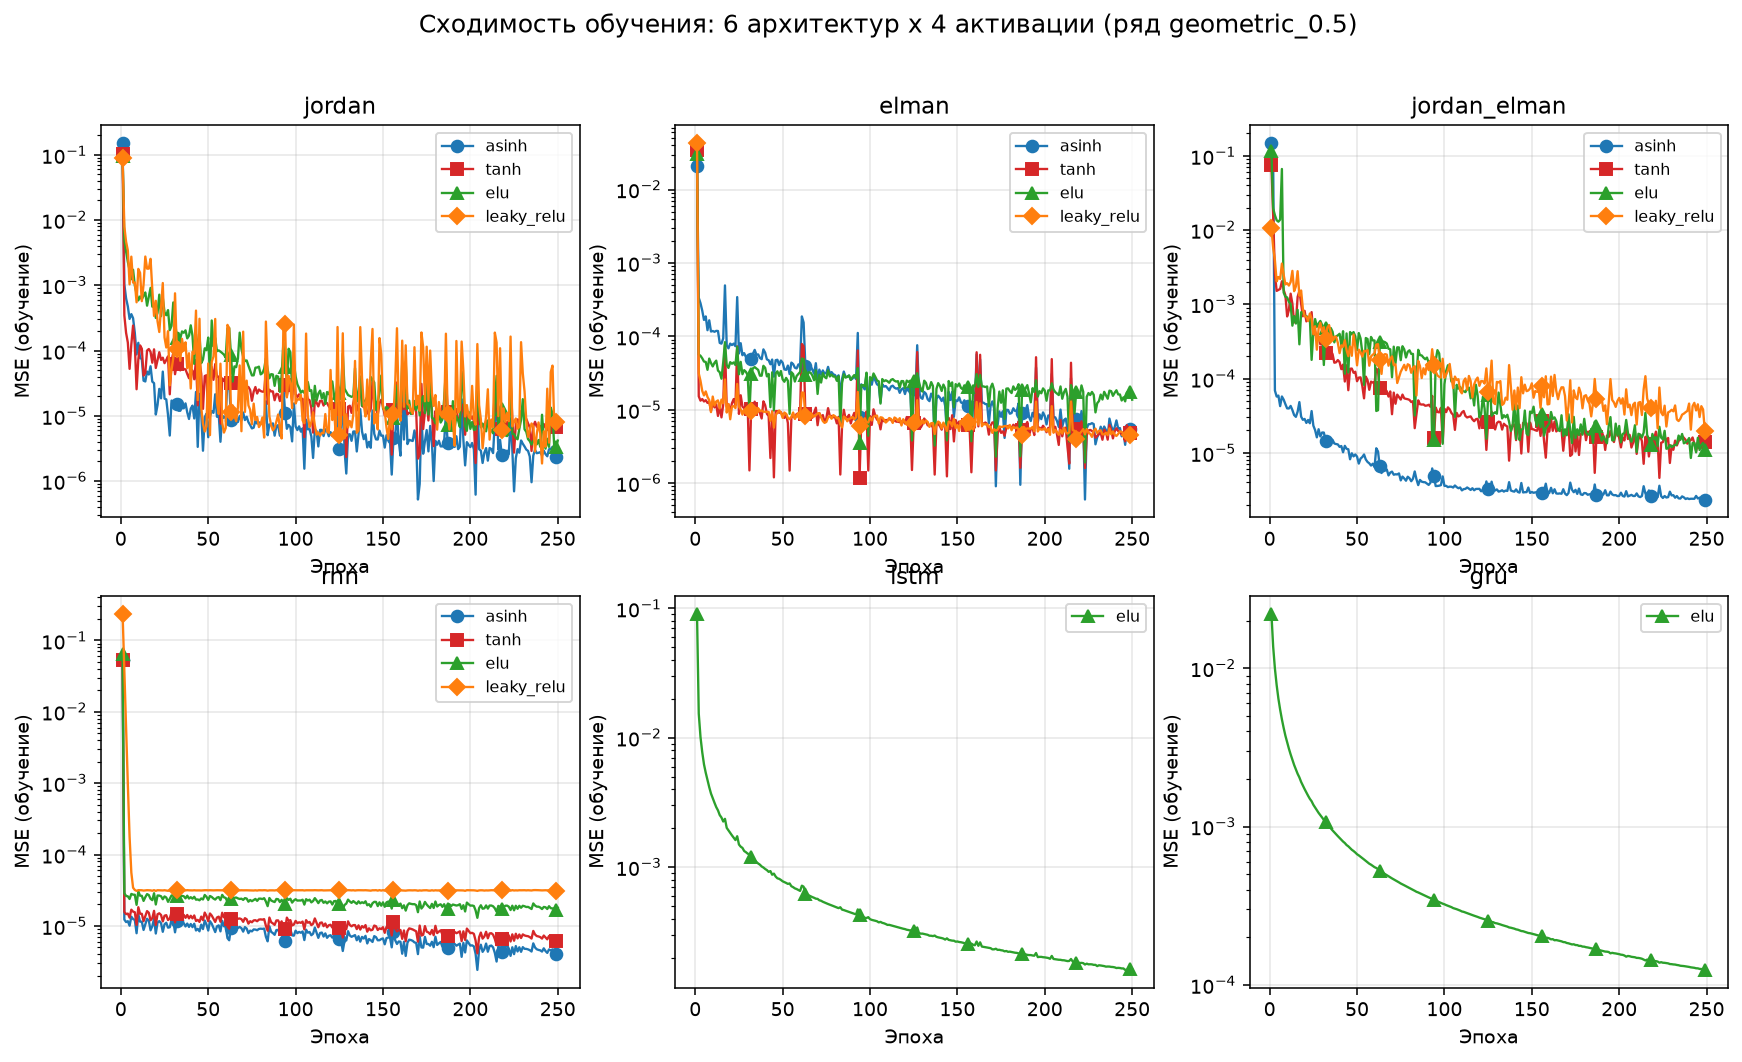
\includegraphics[width=0.98\textwidth]{arch_convergence.png}
	\caption{Сходимость обучения: 6 архитектур $\times$ 4 активации (ряд $0{,}5^n$)}
	\label{fig:conv}
\end{figure}

Все архитектуры сходятся, функция потерь убывает практически до нуля. Сводка по лучшей активации для каждой архитектуры приведена в таблице~\ref{tab:arch}.

\begin{table}[H]
	\centering
	\caption{Лучшая активация и качество прогноза по архитектурам (ряд $0{,}5^n$)}
	\label{tab:arch}
	\begin{tabular}{lccc}
		\hline
		Архитектура & Активация & $\mathrm{MSEn}$ & $\mathrm{MSE}$ \\
		\hline
		Джордан      & Leaky ReLU & $2{,}2 \cdot 10^{-4}$ & $5{,}4 \cdot 10^{-5}$ \\
		Элман        & tanh       & $9{,}0 \cdot 10^{-6}$ & $2{,}2 \cdot 10^{-6}$ \\
		Джордан--Элман & arcsinh  & $9{,}9 \cdot 10^{-6}$ & $2{,}5 \cdot 10^{-6}$ \\
		КП (rnn)     & arcsinh    & $3{,}9 \cdot 10^{-6}$ & $9{,}8 \cdot 10^{-7}$ \\
		LSTM (ДКП)   & ELU        & $5{,}9 \cdot 10^{-4}$ & $1{,}5 \cdot 10^{-4}$ \\
		GRU          & ELU        & $3{,}4 \cdot 10^{-4}$ & $8{,}5 \cdot 10^{-5}$ \\
		\hline
	\end{tabular}
\end{table}

Простые рекуррентные архитектуры (Элман, Джордан, КП) достигают наименьшей ошибки; LSTM и GRU из-за множества ворот сходятся медленнее, но также обеспечивают малый $\mathrm{MSEn}$.

\subsubsection{Влияние размера окна}

На рисунке~\ref{fig:window} приведена зависимость $\mathrm{MSE}$ прогноза от размера скользящего окна $w$ (сеть Элмана, arcsinh).

\begin{figure}[H]
	\centering
	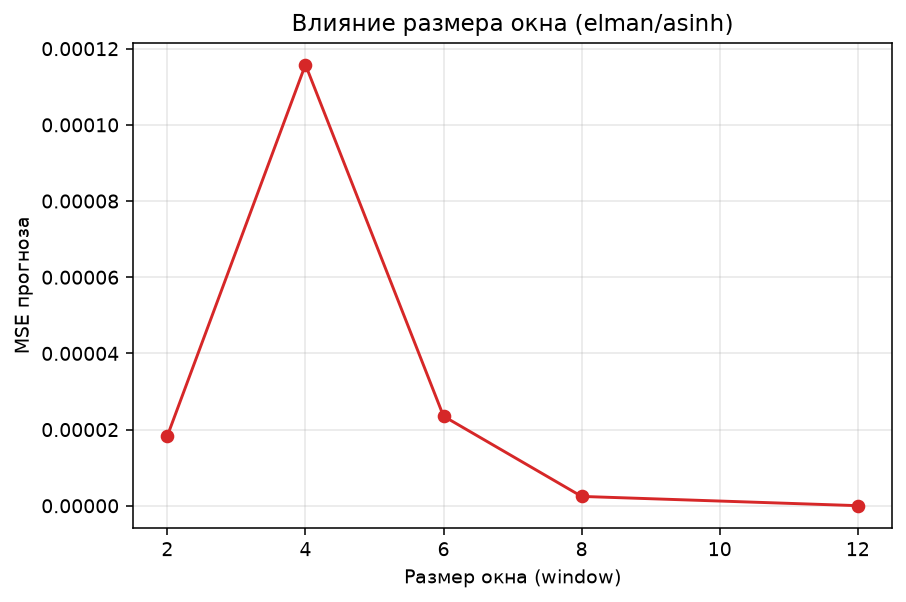
\includegraphics[width=0.7\textwidth]{window_sweep.png}
	\caption{Зависимость ошибки прогноза от размера окна}
	\label{fig:window}
\end{figure}

С ростом размера окна ошибка в среднем убывает и достигает минимума при наибольшем окне: $\mathrm{MSE}$ при $w = 2 \Rightarrow 1{,}8 \cdot 10^{-5}$, $w = 6 \Rightarrow 2{,}4 \cdot 10^{-5}$, $w = 8 \Rightarrow 2{,}5 \cdot 10^{-6}$, $w = 12 \Rightarrow 2{,}8 \cdot 10^{-8}$. Зависимость немонотонна на малых окнах (при $w = 4$ ошибка составила $1{,}2 \cdot 10^{-4}$), но общий тренд~\mdash  убывание: больше окно~\mdash  больше контекста для предсказания следующего отсчёта.

\subsubsection{Влияние числа контекстных нейронов}

На рисунке~\ref{fig:context} приведены зависимости $\mathrm{MSE}$ от $C$ для сетей Джордана, Элмана и Джордана~--~Элмана.

\begin{figure}[H]
	\centering
	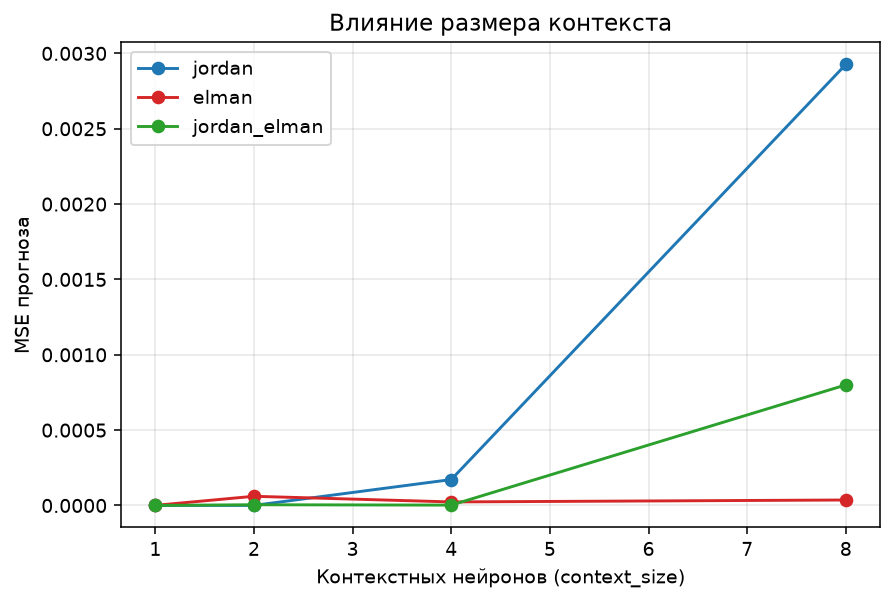
\includegraphics[width=0.7\textwidth]{context_sweep.png}
	\caption{Зависимость ошибки прогноза от числа контекстных нейронов}
	\label{fig:context}
\end{figure}

Наилучшие результаты достигаются при малом числе контекстных нейронов ($C = 1$--$2$, где $\mathrm{MSE} \sim 10^{-7}$--$10^{-6}$); при увеличении $C$ ошибка возрастает (у сети Джордана~\mdash  с $4{,}3 \cdot 10^{-7}$ при $C = 1$ до $2{,}9 \cdot 10^{-3}$ при $C = 8$, у Джордана~--~Элмана~\mdash  до $8{,}0 \cdot 10^{-4}$), поскольку избыточный контекст «зашумляет» вход и усложняет обучение на коротком ряду.

\subsubsection{Влияние размера скрытого слоя}

На рисунке~\ref{fig:hidden} приведена зависимость $\mathrm{MSE}$ от $H$ (сеть КП, arcsinh).

\begin{figure}[H]
	\centering
	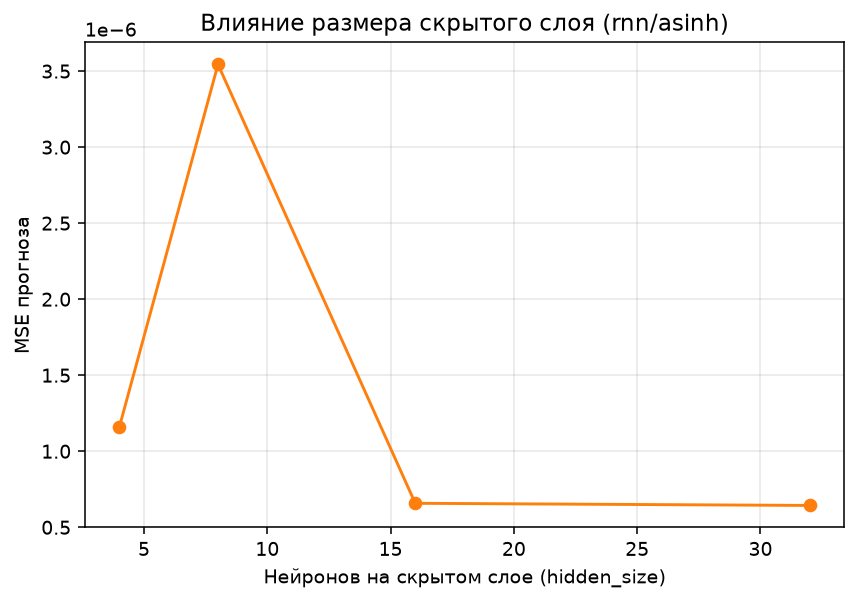
\includegraphics[width=0.7\textwidth]{hidden_sweep.png}
	\caption{Зависимость ошибки прогноза от числа нейронов скрытого слоя}
	\label{fig:hidden}
\end{figure}

Ошибка остаётся малой ($\mathrm{MSE} \sim 6 \cdot 10^{-7}$--$4 \cdot 10^{-6}$) во всём диапазоне $H = 4$--$32$: для простого ряда достаточно малого скрытого слоя, избыточные нейроны не дают устойчивого выигрыша.

\subsubsection{Эффект линейной активации эффекторов}

На рисунке~\ref{fig:effector} приведено сравнение качества при линейном ($g(u) = u$) и нелинейном эффекторе для всех архитектур (скрытый слой~\mdash  arcsinh).

\begin{figure}[H]
	\centering
	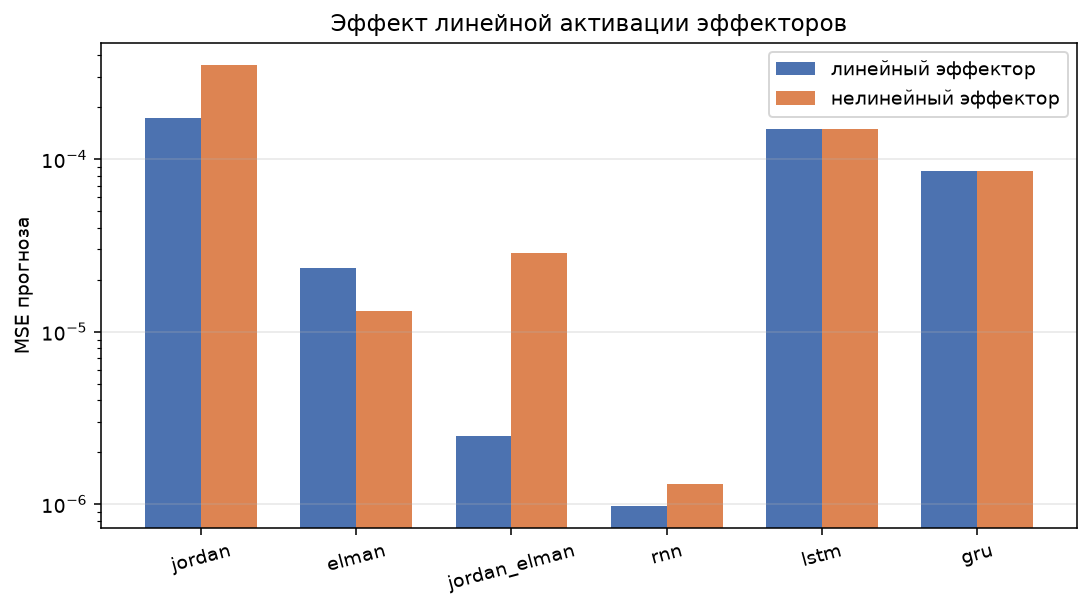
\includegraphics[width=0.85\textwidth]{effector_linear.png}
	\caption{Сравнение линейного и нелинейного эффекторов}
	\label{fig:effector}
\end{figure}

Разница невелика (обе ошибки малы), но заметна. Для сети Элмана нелинейный эффектор точнее ($1{,}3 \cdot 10^{-5}$ против $2{,}4 \cdot 10^{-5}$), для Джордана и Джордана~--~Элмана~\mdash  наоборот, линейный ($1{,}7 \cdot 10^{-4}$ против $3{,}5 \cdot 10^{-4}$ и $2{,}5 \cdot 10^{-6}$ против $2{,}8 \cdot 10^{-5}$ соответственно); у сети КП эффект пренебрежимо мал ($1{,}0 \cdot 10^{-6}$ против $1{,}3 \cdot 10^{-6}$). Для LSTM и GRU эффектор всегда ELU (требование методички), поэтому столбцы совпадают.

\subsubsection{Зануление контекстных нейронов}

На рисунке~\ref{fig:zero} приведены кривые обучения при \texttt{zero\_context} $=$ True (зануление контекста в начале каждой эпохи) и False (перенос контекста между эпохами).

\begin{figure}[H]
	\centering
	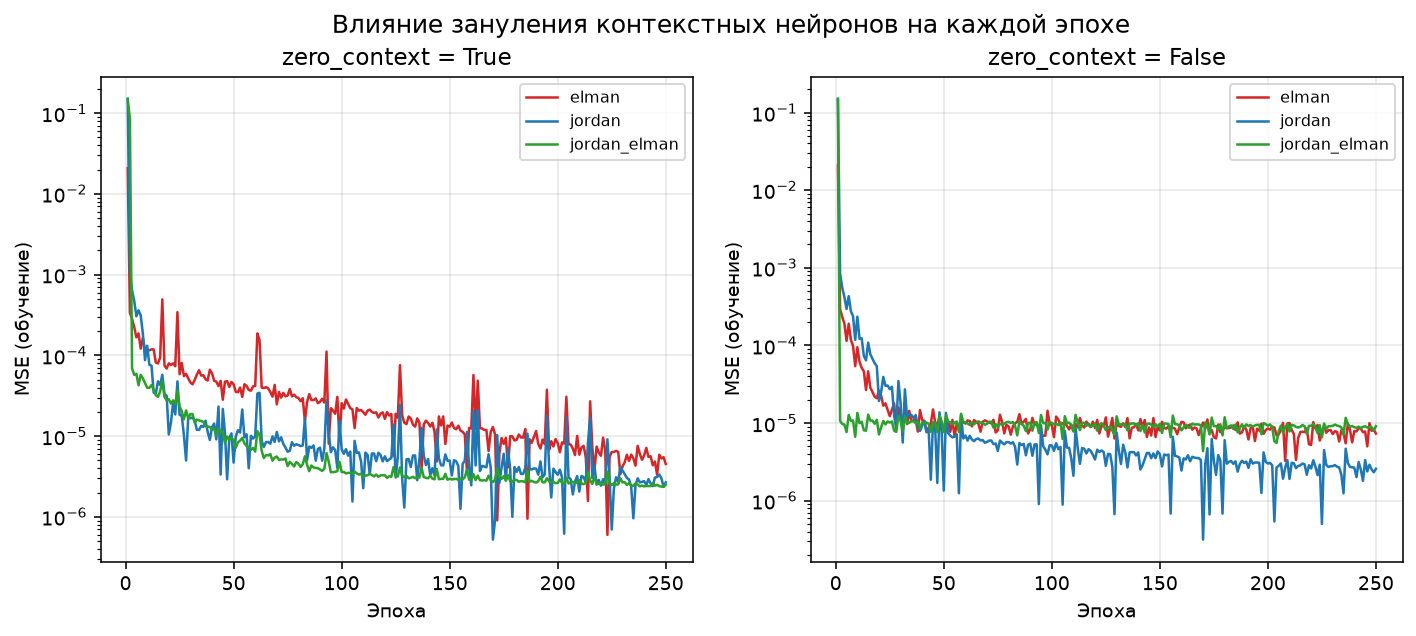
\includegraphics[width=0.95\textwidth]{zero_context.png}
	\caption{Влияние зануления контекстных нейронов на каждой эпохе}
	\label{fig:zero}
\end{figure}

Зануление контекста в начале эпохи устойчиво улучшает качество: для сети Джордана~--~Элмана $\mathrm{MSE}$ снижается с $2{,}4 \cdot 10^{-1}$ (перенос контекста) до $2{,}5 \cdot 10^{-6}$ (зануление), для Элмана~\mdash  с $1{,}2 \cdot 10^{-4}$ до $2{,}4 \cdot 10^{-5}$, для Джордана~\mdash  с $1{,}9 \cdot 10^{-4}$ до $1{,}7 \cdot 10^{-4}$. Это объясняется тем, что «запылённый» контекст из нерелевантного окна ухудшает начальное состояние обучения.

\subsubsection{Начальные веса эффекторов}

На рисунке~\ref{fig:einit} приведена зависимость $\mathrm{MSE}$ от начальной инициализации весов эффекторного нейрона для сетей Джордана и Джордана~--~Элмана.

\begin{figure}[H]
	\centering
	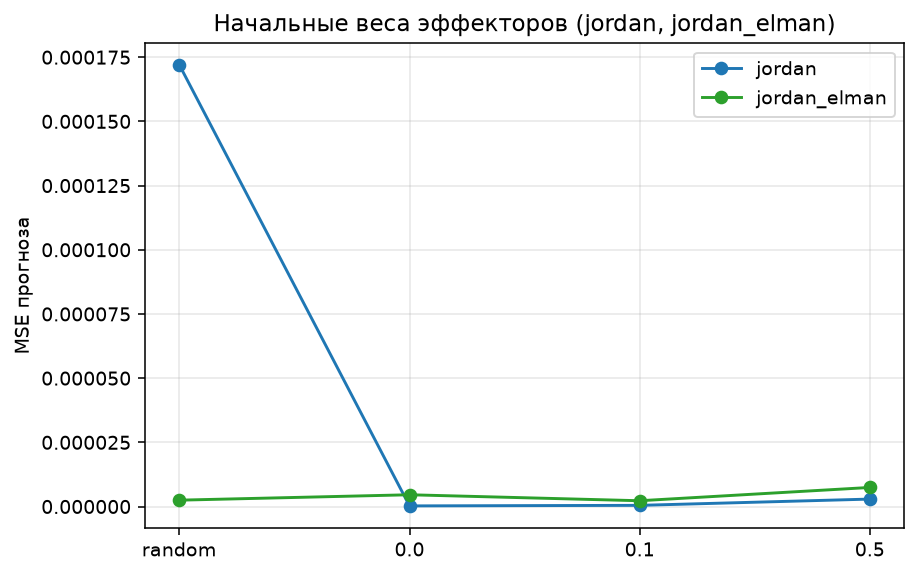
\includegraphics[width=0.7\textwidth]{effector_init.png}
	\caption{Влияние начальных весов эффекторных нейронов}
	\label{fig:einit}
\end{figure}

Инициализация весов эффектора влияет по-разному. Для сети Джордана нулевая инициализация $W_{ho}$ даёт $\mathrm{MSE} = 2{,}4 \cdot 10^{-7}$ против $1{,}7 \cdot 10^{-4}$ при случайной~\mdash  выигрыш в $\approx 3$ порядка; значение $0{,}1$ также эффективно ($4{,}5 \cdot 10^{-7}$), а $0{,}5$ уступает ($2{,}9 \cdot 10^{-6}$). Для сети Джордана~--~Элмана управляемая инициализация даёт скромный эффект: значение $0{,}1$ ($2{,}3 \cdot 10^{-6}$) лишь немного лучше случайной ($2{,}5 \cdot 10^{-6}$), а нулевая ($4{,}6 \cdot 10^{-6}$) и $0{,}5$ ($7{,}4 \cdot 10^{-6}$)~\mdash  хуже. Таким образом, настраиваемые начальные веса эффекторов (требование методички) полезны прежде всего для сети Джордана.

\subsubsection{Многомерный прогноз}

На рисунке~\ref{fig:forecast} приведены примеры многошагового прогноза (8 отсчётов вперёд) скользящим окном с сохранением контекста на шести рядах; для каждого показана лучшая архитектура.

\begin{figure}[H]
	\centering
	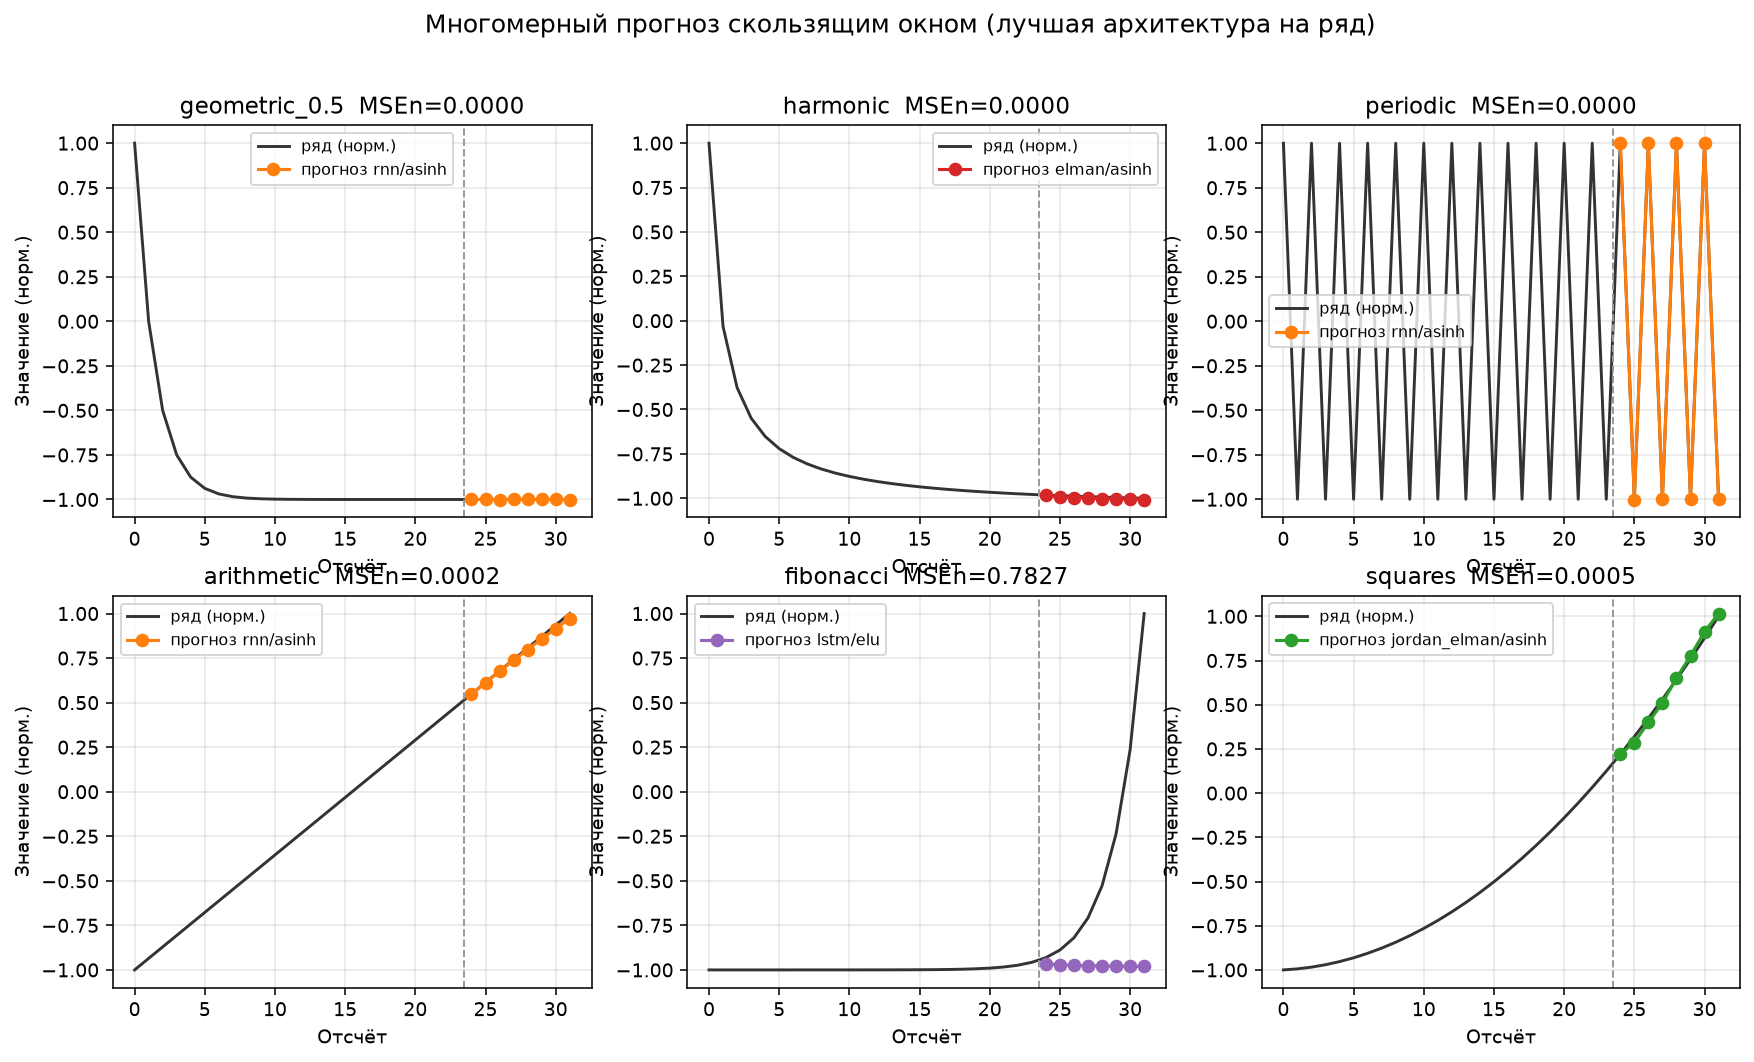
\includegraphics[width=0.98\textwidth]{forecast_multi.png}
	\caption{Многомерный прогноз скользящим окном (лучшая архитектура на ряд)}
	\label{fig:forecast}
\end{figure}

Для «мягких» рядов (геометрическая прогрессия $0{,}5^n$, гармонический ряд, периодическая последовательность, арифметическая прогрессия, квадраты) прогноз практически совпадает с фактом ($\mathrm{MSEn} \lesssim 10^{-3}$). Для быстро растущих (факториал, числа Белла, $2^n$, Фибоначчи) и апериодической последовательности ошибка существенна ($\mathrm{MSEn} \approx 0{,}4$--$0{,}7$): сеть обучается в диапазоне $[-1, 1]$ и не умеет экстраполировать сверхлинейный рост за пределы обучающей выборки. Сводная таблица~\ref{tab:summary} приводит лучшую архитектуру для каждого ряда.

\begin{table}[H]
	\centering
	\caption{Лучшая архитектура/активация для каждого ряда (горизонт 8 отсчётов)}
	\label{tab:summary}
	\begin{tabular}{llcl}
		\hline
		Ряд & Архитектура & Активация & $\mathrm{MSEn}$ \\
		\hline
		$0{,}5^n$            & КП (rnn)     & ELU        & $0{,}0000$ \\
		Гармонический $1/n$  & Элман        & tanh       & $0{,}0000$ \\
		$0{,}2^n$            & КП (rnn)     & Leaky ReLU & $0{,}0000$ \\
		Периодическая        & КП (rnn)     & Leaky ReLU & $0{,}0000$ \\
		Арифметическая       & КП (rnn)     & arcsinh    & $0{,}0002$ \\
		Квадраты             & Джордан--Элман & arcsinh  & $0{,}0005$ \\
		Нечётные             & КП (rnn)     & arcsinh    & $0{,}0002$ \\
		Апериодическая       & GRU          & ELU        & $0{,}4445$ \\
		$2^n$                & Джордан--Элман & tanh     & $0{,}6337$ \\
		Числа Белла          & Джордан--Элман & arcsinh  & $0{,}4845$ \\
		Факториал            & Джордан--Элман & arcsinh  & $0{,}4833$ \\
		Фибоначчи            & Элман        & ELU        & $0{,}7053$ \\
		\hline
	\end{tabular}
\end{table}

\subsection{Ответы на вопросы}

\begin{enumerate}
	\item \textbf{Что такое рекуррентная сеть?} НС с обратными (рекуррентными) связями, удерживающая внутреннее состояние (контекст), благодаря чему обрабатывает последовательности и учитывает зависимость выхода от предыдущих входов~\cite{haykin}.
	\item \textbf{Чем сеть Элмана отличается от сети Джордана?} У Элмана контекст формируется из скрытого слоя ($c_{t+1} = h_t$), у Джордана~\mdash  из выхода эффектора ($c_{t+1} = y_t$). Сеть Джордана--Элмана объединяет оба источника.
	\item \textbf{Что такое долговременная кратковременная память?} Архитектура LSTM с воротами (вход, забвение, выход) и ячейным состоянием $c_t$, позволяющая сохранять информацию на длинных интервалах и избегать затухания градиентов.
	\item \textbf{Зачем нужна функция активации эффектора?} Она отображает выход скрытого слоя в область значений ряда; линейная активация ($g(u)=u$) уместна для регрессии, ELU~\mdash  требование методички для LSTM/GRU.
	\item \textbf{Как реализуется многомерный прогноз?} Методом скользящего окна: сеть «раскатывается» на опорном окне, затем предыдущий прогноз подаётся на вход с сохранённым контекстом $H$ раз ($H \ge 3$).
	\item \textbf{Влияет ли зануление контекста на эпохе?} Да, зануление в начале эпохи улучшает устойчивость обучения (см. рис.~\ref{fig:zero}), устраняя перенос нерелевантного контекста между эпохами.
	\item \textbf{Почему ряд нормализуется в $[-1, 1]$?} Выходы эффекторов малой сети ограничены по амплитуде; min--max нормализация отображает ряд в рабочую область сети, а обратное преобразование возвращает исходные единицы.
	\item \textbf{Какие ряды труднее прогнозировать?} Быстрорастущие (факториал, числа Белла, $2^n$, Фибоначчи) и апериодические: сеть, обученная в $[-1, 1]$, плохо экстраполирует сверхлинейный рост за пределы обучающей выборки (см. табл.~\ref{tab:summary}).
\end{enumerate}
